\documentclass[letterpaper,11pt]{article}
\oddsidemargin -1.0cm \textwidth 17.5cm

\usepackage[utf8]{inputenc}
\usepackage[activeacute,spanish, es-lcroman]{babel}
\decimalpoint
\usepackage{amsfonts,setspace}
\usepackage{amsmath}
\usepackage{amssymb, amsmath, amsthm}
\usepackage{comment}
\usepackage{float}
\usepackage{amssymb}
\usepackage{dsfont}
\usepackage{anysize}
\usepackage{multicol}
\usepackage{enumerate}
\usepackage{graphicx}
\usepackage[left=1.5cm,top=2cm,right=1.5cm, bottom=1.7cm]{geometry}
\setlength\headheight{1.5em} 
\usepackage{fancyhdr}
\usepackage{multicol}
\usepackage{hyperref}
\usepackage{wrapfig}
\usepackage{subcaption}
\usepackage{siunitx}
\usepackage{cancel}
\usepackage{mdwlist}
\usepackage{svg}
\usepackage{tcolorbox}
\pagestyle{fancy}
\fancyhf{}
\renewcommand{\labelenumi}{\normalsize\bfseries P\arabic{enumi}.}
\renewcommand{\labelenumii}{\normalsize\bfseries (\alph{enumii})}
\renewcommand{\labelenumiii}{\normalsize\bfseries \roman{enumiii})}


\begin{document}

\fancyhead[L]{\itshape{Facultad de Ciencias F\'isicas y Matem\'aticas}}
\fancyhead[R]{\itshape{Universidad de Chile}}

\begin{minipage}{11.5cm}
    \begin{flushleft}
        \hspace*{-0.6cm}\textbf{FI1000-1 Introducción a la Física Clásica}\\
        \hspace*{-0.6cm}\textbf{Profesora:} Jocelyn Dunstan\\
        \hspace*{-0.6cm}\textbf{Auxiliar:} Alejandro Silva\\
        \hspace*{-0.6cm}\textbf{Ayudantes:} Macarena Muñoz \& Catalina Vargas\\
    \end{flushleft}
\end{minipage}

\begin{picture}(2,3)
    \svgpath{../}  % descomentar si se agrega a carpeta "auxiliares"/"ejercicios"
    \put(366, 10){\includesvg[scale=0.31]{img/dfi.svg}}
\end{picture}

\begin{center}
	\LARGE\textbf{Auxiliar \#13}\\
	\Large{Estática 2 e Hidrostática}
\end{center}

\vspace{-1cm}
\begin{enumerate}\setlength{\itemsep}{0.4cm}

\rfoot[]{pág. \thepage}

\item[]

\item Considere una semiesfera de radio $R$ de masa $M$ que se encuentra sobre una superficie horizontal y apoyada contra una pared tal como se muestra en la figura adjunta. El centro de masas de una semiesfera homogénea queda sobre el eje de simetría y a una distancia ${b} = 3 R / 8$ de la base. Suponga que, entre la semiesfera y el suelo el coeficiente de roce estático es $\mu = 3 / 16$, mientras que entre la pared y la semiesfera el roce es nulo.

\begin{multicols}{2}
    \begin{enumerate}
        \item Realice un diagrama de cuerpo libre para la semiesfera.
        \item Encuentre la magnitud y dirección del torque, respecto al punto de apoyo $P$, ejercido por la fuerza de gravedad cuando la semiesfera está ladeada en un ángulo $\beta$.
        \item Encuentre la fuerza de roce entre la semi-esfera y el suelo
        \item Encuentre el ángulo de inclinación mínimo $\beta_{min}$ posible para que la semiesfera no resbale.
    \end{enumerate}
    
    \columnbreak
    
    \begin{figure}[H]
        \centering
        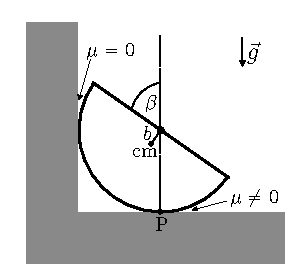
\includegraphics[width=0.6\linewidth]{2020-1/Imágenes/aux Extra-C2/semiesfera-torque.pdf}
    \end{figure}
\end{multicols}

\item Una varilla de largo $L$ y densidad $\rho_1$ flota en un líquido de densidad $\rho_0$ $\left(\rho_0 > \rho_1\right)$. Un extremo de la varilla se amarra a un hilo a una profundidad $h$.

\begin{multicols}{2}
    \begin{enumerate}
        \item Determine el ángulo $\alpha$
        \item ¿Cuál es el mínimo valor de h para el cual la varilla se mantiene en posición vertical?
        \item Si $A$ es la sección transversal de la varilla, encuentre la tensión del hilo
    \end{enumerate}
    
    \columnbreak
    
    \begin{figure}[H]
        \centering
        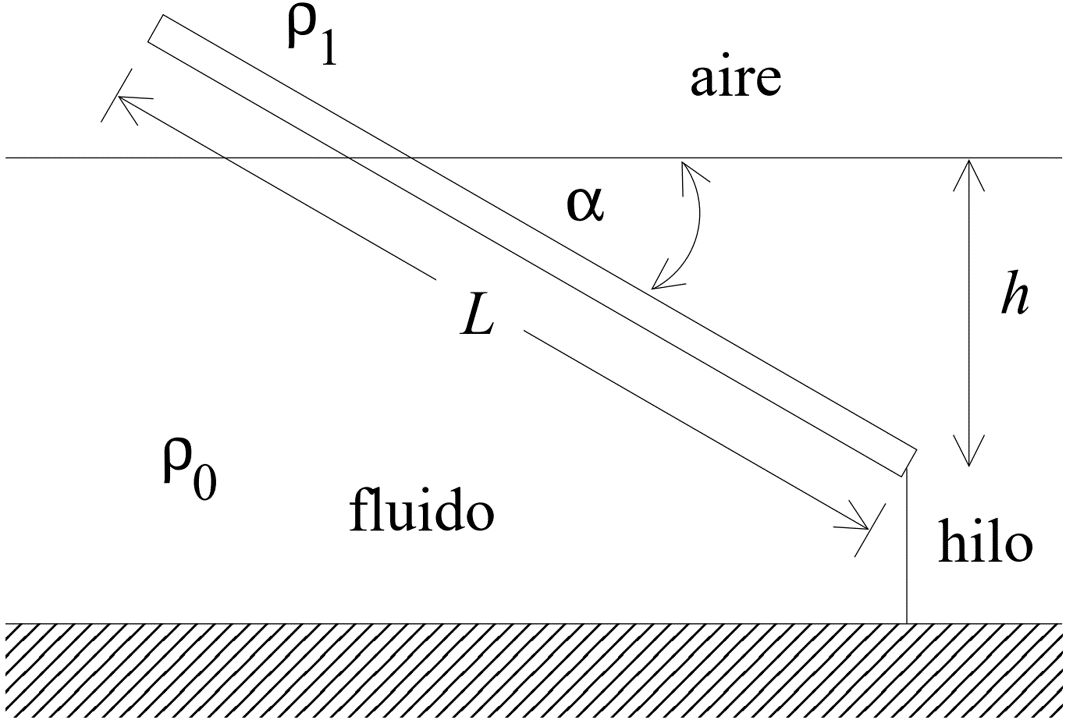
\includegraphics[width=0.55\linewidth]{2021-2/img/aux13/p1.png}
    \end{figure}
\end{multicols}

\item Un tubo en U abierto en ambos extremos se llena parcialmente con mercurio. A continuación se vierten $m=\SI{100}{\g}$ de agua en el brazo derecho, como se muestra en la figura. Si el brazo izquierdo del tubo tiene un área de sección transversal $A_1=\SI{10}{\cm^2}$ y el brazo derecho tiene un área de sección transversal $A_2=\SI{5}{\cm^2}$, determine:
\begin{multicols}{2}
    \begin{enumerate}
        \item La longitud de la columna de agua en el brazo derecho del tubo
        \item Si la densidad del mercurio es $\rho_{Hg}~=~\SI{13.6}{\g/\cm^3}$, ¿qué distancia h se eleva el mercurio en el brazo izquierdo?
    \end{enumerate}
    \columnbreak
    \begin{figure}[H]
        \centering
        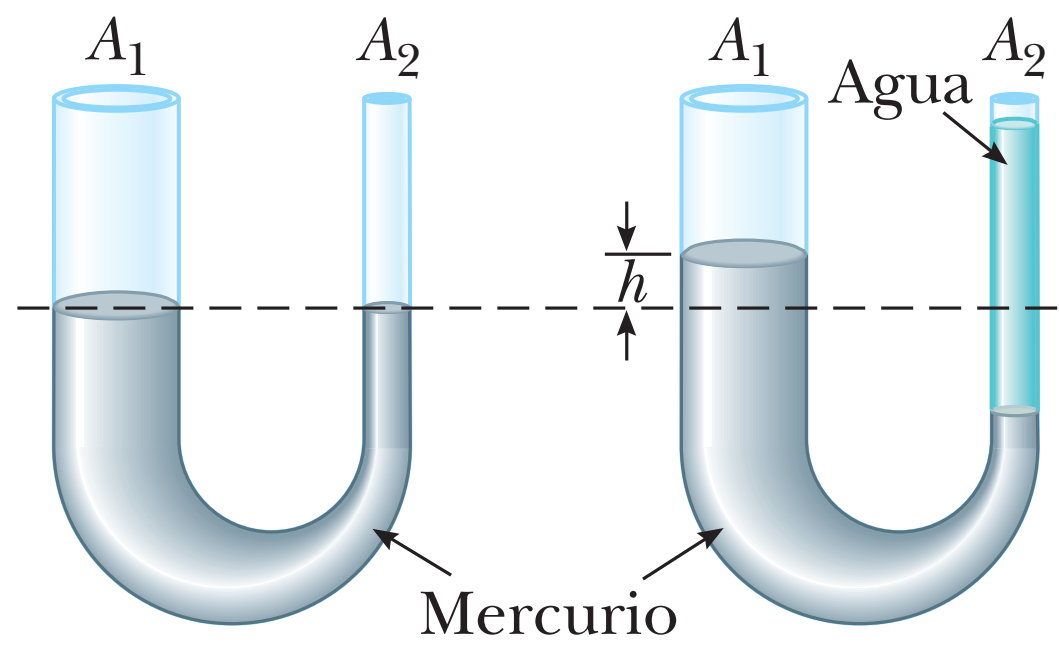
\includegraphics[width=0.5\linewidth]{2021-2/img/aux13/p2.png}
    \end{figure}
\end{multicols}

% Para imágenes vectoriales -> el texto tiene que estar en LaTeX
% \begin{figure}[htbp]
%   \centering
%   \svgpath{../Imagenes/ejercicios}  -> .. irse pa'trás 
%   \includesvg{ej5.svg}
% \end{figure}

\end{enumerate}
\end{document}